% This file was created by matlab2tikz.
%
%The latest updates can be retrieved from
%  http://www.mathworks.com/matlabcentral/fileexchange/22022-matlab2tikz-matlab2tikz
%where you can also make suggestions and rate matlab2tikz.
%
\documentclass[tikz]{standalone}
\usepackage[T1]{fontenc}
\usepackage[utf8]{inputenc}
\usepackage{pgfplots}
\usepackage{grffile}
\pgfplotsset{compat=newest}
\usetikzlibrary{plotmarks}
\usepgfplotslibrary{patchplots}
\usepackage{amsmath}
\usetikzlibrary{decorations.markings}
\begin{document}

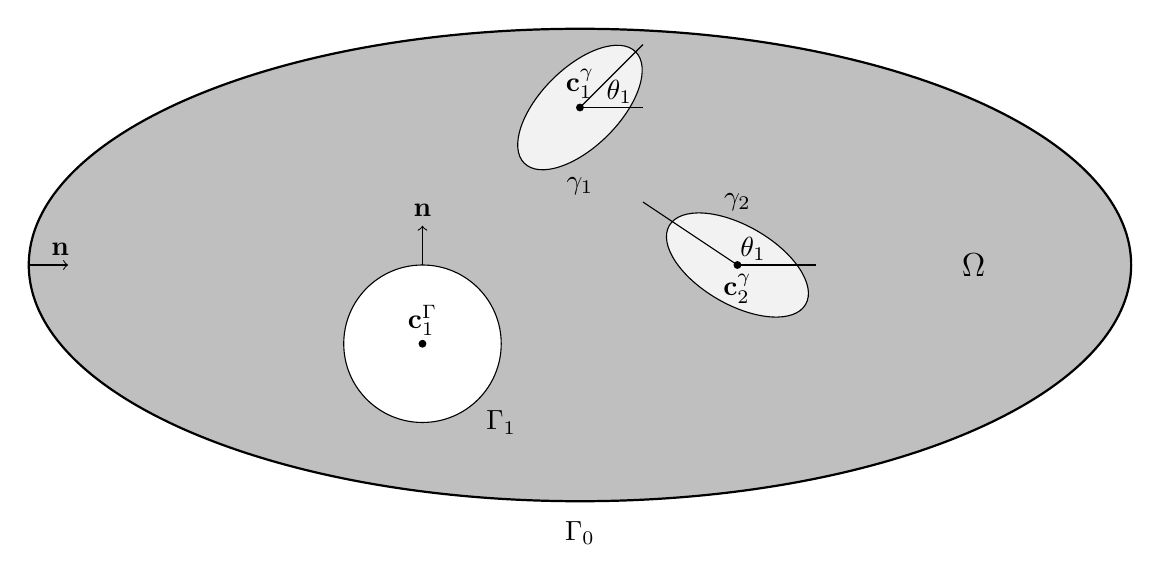
\begin{tikzpicture}
	\draw[fill=lightgray, draw=black, thick](0,0) circle[x radius=7, y radius=3];
	\draw[fill=lightgray!20!white] (0,2) circle [x radius=0.5, y radius=1, rotate around={-45:(0,0)}];
	\draw[fill=lightgray!20!white] (2,0) circle [x radius=0.5, y radius=1, rotate around={60:(0,0)}];
	\draw[fill=white] (-2,-1) circle [x radius=1, y radius=1];
	 \fill(0,2)circle(0.05);
	 \draw(0,2.3) node {$\mathbf{c}^\gamma_1$};
	\fill(2,0)circle(0.05);
	 \draw(2,-0.3) node {$\mathbf{c}^\gamma_2$};
	 \fill(-2,-1)circle(0.05);
	 \draw(-2,-0.7) node {$\mathbf{c}^\Gamma_1$};
	 \draw(0,1) node {$\gamma_1$};
	 \draw(2,0.8) node {$\gamma_2$};
	 \draw(-1,-2) node {$\Gamma_1$};
	 \draw(0,-3.4) node {$\Gamma_0$};
	 \draw(0,2)--(0.8,2.8);
	 \draw(0,2)--(0.8,2);
	  \draw(0.5,2.2) node {$\theta_1$};
	  \draw(2,0)--(0.8,0.8);
	 \draw(2,0)--(3,0);
	  \draw(2.2,0.2) node {$\theta_1$};
	  \draw[->](-7,0)--(-6.5,0);
	   \draw[->](-2,0)--(-2,0.5);
	    \draw(-6.6,0.2) node {$\mathbf{n}$};
	      \draw(-2,0.7) node {$\mathbf{n}$};
	          \draw(5,0) node {\large$\Omega$};
\end{tikzpicture}
\end{document}